\definecolor{lavander}{cmyk}{0,0.48,0,0}
\definecolor{violet}{cmyk}{0.79,0.88,0,0}
\definecolor{burntorange}{cmyk}{0,0.52,1,0}

\def\lav{lavander!90}
\def\oran{orange!30}

\tikzstyle{contingency}=[draw,circle,violet,bottom color=\lav,
                  top color= white, text=violet,minimum width=50pt]
\tikzstyle{base}=[draw,circle,burntorange, left color=\oran,
                       text=violet,minimum width=50pt]

\tikzstyle{time}=[draw,circle,blue,text=violet,minimum width=2pt]
\tikzstyle{tbase}=[draw,circle,burntorange, left color=\oran,
                            text=violet,minimum width=2pt]
                       
\tikzstyle{cedge}=[color=red]

\begin{figure}[h!]
\centering
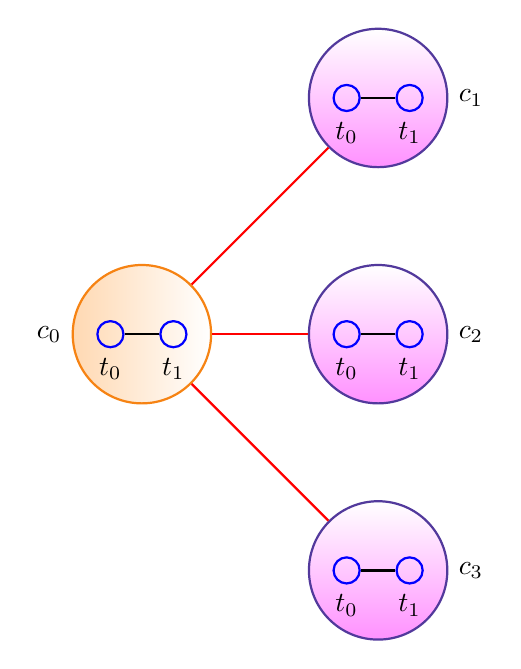
\begin{tikzpicture}[auto, thick]
  % Place base case
  \node[base,label=left:$c_0$] (base) at (0,0) {};
  \node[time,label=below:$t_0$] (c0t0) at (-0.4,0) {};
  \node[time,label=below:$t_1$] (c0t1) at (0.4,0) {};
  
  \node[contingency,label=right:$c_1$] (c1) at (3,3) {};
  \node[time,label=below:$t_0$] (c1t0) at (2.6,3) {};
  \node[time,label=below:$t_1$] (c1t1) at (3.4,3) {};

  \node[contingency,label=right:$c_2$] (c2) at (3,0) {};
  \node[time,label=below:$t_0$] (c2t0) at (2.6,0) {};
  \node[time,label=below:$t_1$] (c2t1) at (3.4,0) {};

  
  \node[contingency,label=right:$c_3$] (c3) at (3,-3) {};
  \node[time,label=below:$t_0$] (c3t0) at (2.6,-3) {};
  \node[time,label=below:$t_1$] (c3t1) at (3.4,-3) {};
  
  \path (c0t0) edge (c0t1);
  \path (c1t0) edge (c1t1);
  \path (c2t0) edge (c2t1);
  \path (c3t0) edge (c3t1);
  
  \path[cedge] (base) edge (c1);
  \path[cedge] (base) edge (c2);
  \path[cedge] (base) edge (c3);  
  
  
%  \foreach \place/\name in {{(0,-1)/a}, {(2,0)/b}, {(2,2)/c}, {(0,2)/d},
%           {(-2,0)/e}}
%    \node[superpeers] (\name) at \place {a};
%  \foreach \source/\dest in {a/b, a/c, a/d, b/c, c/d,a/e,d/e}
%    \path (\source) edge (\dest);
   %
   % Place normal peers
%  \foreach \pos/\i in {above left of/1, left of/2, below left of/3}
%    \node[peers, \pos = e] (e\i) {};
%   \foreach \speer/\peer in {e/e1,e/e2,e/e3}
%    \path (\speer) edge (\peer);
   %
%   \foreach \pos/\i in {above right of/1, right of/2, below right of/3}
%    \node[peers, \pos =b ] (b\i) {};
%   \foreach \speer/\peer in {b/b1,b/b2,b/b3}
%   \path (\speer) edge (\peer);
   %
%   \node[peers, above of=d] (d1){};
%   \path (d) edge (d1);
   %
%   \foreach \pos/\i in {below left of/1, below of/2}
%   \node[peers, \pos =a ] (a\i) {};
%   \foreach \speer/\peer in {a/a1,a/a2}
%   \path (\speer) edge (\peer);

\end{tikzpicture}
\caption{Multi-period contingency constrained optimal power flow example with two contingencies $c_0$ and $c_1$, each with two time-periods $t_0$, $t_1$. State $c_0$ represents the base case (no contingency) case. The contingency states $c_1$,$c_2$,$c_3$ are coupled with the no-contingency state $c_0$. The {\textcolor{red}{red}} line denotes the coupling between the contingencies.}
\label{fig:ctopflow}
\end{figure}